\documentclass[11pt]{article}
\usepackage[a4paper,top=3cm,bottom=3cm,left=2.5cm,right=2.5cm]{geometry}
\usepackage[italian]{babel}
\usepackage[utf8x]{inputenc}
\usepackage {caption}
\usepackage {amsmath}
\usepackage {kbordermatrix}

\usepackage {url}
\usepackage {multirow}
\usepackage {booktabs}
\usepackage {fixltx2e}
\usepackage {float}
\usepackage {graphicx}
\usepackage {cite}
\usepackage {listings}
\usepackage {color}
\usepackage {xcolor,colortbl}
\usepackage {adjustbox}
\usepackage {array}
\usepackage {svg}
\usepackage {subfig}
\usepackage {amssymb}
\usepackage {hyperref}
\usepackage {tabulary}
\usepackage {tabularx}
\usepackage[T1]{fontenc}
\usepackage{wasysym}
\usepackage{enumitem}
\usepackage{lipsum}
\usepackage{charter} %font

\newcommand{\voceU}[1]{%
	\item #1\dotfill\Square%
}

\newcommand{\voceD}[1]{%
	\item #1\hfill\Square%
}
\hypersetup{colorlinks=true,citecolor=black,linkcolor=black, urlcolor=blue}

\date{}

\renewcommand{\lstlistingname}{Listato}


\lstset{
    language=C,
    basicstyle=\ttfamily,
    breaklines=true,
    frame=single, % draw a frame at the top and bottom of the code block
    tabsize=2, % tab space width
    showstringspaces=false, % don't mark spaces in strings
    numbers=left, % display line numbers on the left
    captionpos=b,
    commentstyle=\color{green}, % comment color
    keywordstyle=\color{blue}, % keyword color
    stringstyle=\color{red} % string color
}

\begin{document}

\title{\textbf{Definizione ed Implementazione di un Sistema di Raccomandazione Distribuito per film
		e Modellazione di Eventi Complessi}}

\author{\\\textit{Prof. Ing.} Tommaso di Noia\\\textit{Prof.ssa} Marina Mongiello \\
	Mauro Losciale\\ 
	Pietro Tedeschi\\}

\clearpage\maketitle
\thispagestyle{empty}

\begin{center}
	
\includegraphics[scale=0.40]{images/poliba.jpg}
\end{center}

{\textbf{\center Logica e Intelligenza Artificiale\\Ingegneria del Software Avanzata\\ Laurea Magistrale in Ingegneria Informatica\\Politecnico di Bari\\A.A 2015 - 2016\\}}

\newpage
\clearpage
\thispagestyle{empty}
\renewcommand\contentsname{Indice}
\tableofcontents
\newpage
\setcounter{page}{1}

\newpage
\section{Introduzione}
\section{Stato dell'arte}

\subsection{Introduzione ai sistemi CEP}
L'incremento dei dispositivi interconnessi e delle applicazioni distribuite, richiede un'elaborazione continua del flusso dati. Esempi di tali applicazioni, vanno dal traffico generato dalle Wireless Sensor Networks (WSN) al flusso dati relativo agli indici finanziari, dal monitoraggio stradale alla Clickstream Analysis. 

Un sistema ad eventi complessi, meglio conosciuto come \textit{Complex Event Processing} (CEP), modella il flusso informativo dei dati, visualizzando gli elementi come notifiche di ciò che sta accadendo nel mondo esterno. I dati vengono rilevati e filtrati utilizzando dei pattern (oppure le \textit{processing rules}), i quali hanno il compito di rappresentare il modello di riferimento con l'informazione da rilevare, per poi farla pervenire alle rispettive parti (ad esempio, i dispositivi che effettuano una sottoscrizione ad un determinato topic nel paradigma \textit{publish-subscribe}). L'obiettivo di un sistema CEP consiste nell'identificare eventi significanti e rispondere ad essi nel più breve tempo possibile.
Un pattern o una regola, può essere definita mediante un linguaggio basato su query, il cosiddetto \textbf{Event Query
	Language}.
\begin{figure}[H]
	\centering
	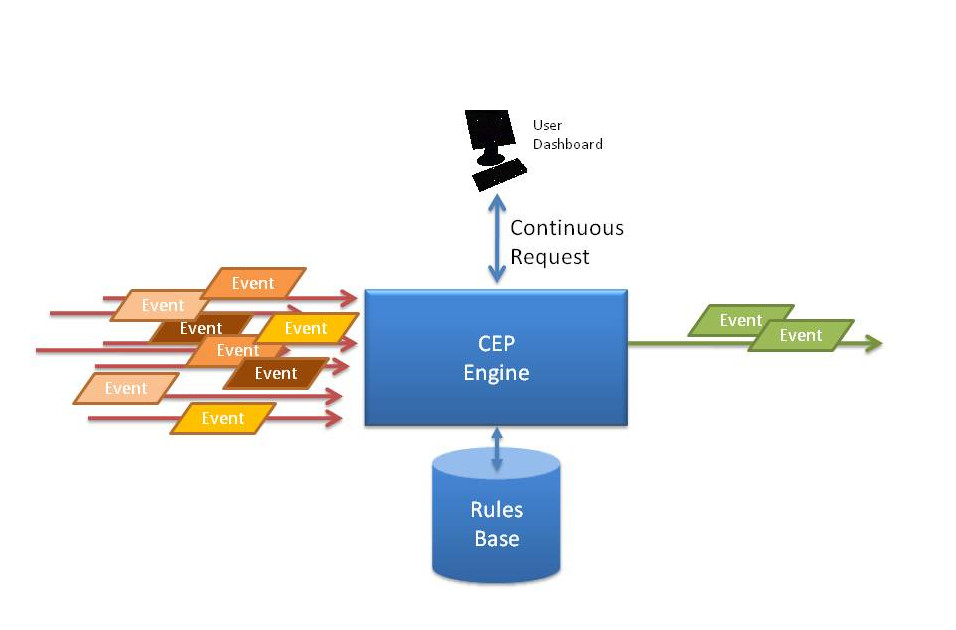
\includegraphics[scale=0.50]{images/CEP2.jpg}
	\caption{Architettura di un Sistema CEP\cite{cepimage}}
	\label{archcep}
\end{figure}

Gli \textbf{Event Query Languages} possono essere raggruppati in tre categorie: Composition Operators, Data Stream Query Languages e
Production Rules. I Composition Operators identificano gli eventi complessi partendo dalla composizione dei singoli eventi, utilizzando operatori quali congiunzione, negazione o di sequenza per la costruzione delle espressioni. Esempi rilevanti sono IBM Active Middleware Technology e ruleCore. 

I \textbf{Data Stream Query Languages} sono basati sul linguaggio SQL; gli stream di dati sono semplicemente tuple convertite per database relazionali, in modo che si possano eseguire query SQL su di esse. E' utile citare i seguenti approcci: CQL, Coral8, StreamBase,
Aleri, Esper e così via.

Le \textbf{Production Rules} specificano le azioni che devono essere eseguite quando il sistema si trova in determinati stati; non è un linguaggio ad eventi, ma costituisce un approccio importante nei sistemi CEP. Un esempio pratico è TIBCO Business Events.

Un altro fattore importante è il tempo. Sono due le parti da considerare quando si parla del tempo, il tempo della finestra ed il tempo dell'evento informativo. Il tempo della finestra mostra gli eventi che vengono esaminati in un determinato intervallo. Il tempo dell'evento invece, porta con se informazioni relative alla data, ora di rilevazione, tempo di transizione, ed intervallo di elaborazione.

I contributi relativi ai sistemi CEP, arrivano da diverse comunità, a partire da quelle che si occupano di sistemi distribuiti, automazione industriale, sistemi di controllo, monitoraggio delle reti, Internet of Things, e middleware in generale.

\begin{figure}[H]
	\centering
	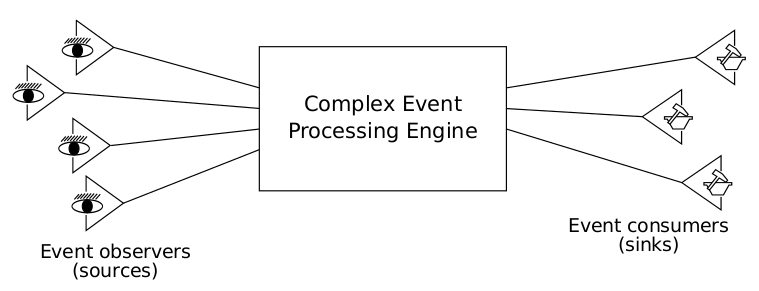
\includegraphics[scale=0.40]{images/CEP.png}
	\caption{Funzionamento di un Sistema CEP (High-Level) \cite{Cugola:2012:PFI:2187671.2187677}}
	\label{funcep}
\end{figure}

Come possiamo vedere dalla Figura \ref{funcep}, viene associata una semantica dettagliata agli elementi informativi da processare. Da una parte abbiamo gli \textbf{Event Observer}, i quali rappresentano la sorgente dei dati e degli eventi da notificare; in seguito abbiamo il \textbf{CEP Engine}, responsabile del filtraggio e della notifica degli eventi ai nodi \textit{sink}, identificati come \textbf{Event Consumers} \cite{Cugola:2012:PFI:2187671.2187677,fulop2010survey}.

\subsection{Sistemi di Raccomandazione}
I sistemi di raccomandazione, raccolgono informazioni sulle preferenze di utente in corrispondenza di un insieme di elementi (ad esempio, film, musica, libri, giochi, viaggi, siti web, applicazioni, gadget). L'informazione può essere acquisita in maniera esplicita (tipicamente ciò viene fatto acquisendo il voto di un utente) o implicitamente (analizzando il comportamento dell'utente, ad esempio musica ascoltata, applicazioni scaricate, siti web visitati, libri letti). Inoltre i sistemi di raccomandazione, possono tener conto anche delle caratteristiche demografiche dell'utente (ad esempio età, nazionalità, sesso); dei contenuti informativi presenti nel mondo del Web 2.0, ad esempio all'interno delle piattaforme di Social Networking, quali follower, followed, twit, like, post; dei dati provenienti dai dispositivi caratterizzanti l'Internet of Things (ad esempio, coordinate GPS, RFID, segnali medici inviati in real-time). 

I sistemi di raccomandazione utilizzano diverse sorgenti informative al fine di fornire all'utente finale una migliore Quality of Experience relativa alla predizione ed alla raccomandazione degli elementi che potrebbero interessargli. La tecnica del Collaborative Filtering (CF), ha un ruolo fondamentale nella raccomandazione, sebbene viene spesso usata anche con altre tecniche di filtraggio basate sul contenuto o basate sulla conoscenza. Il CF si basa sulla cronologia decisionale dell'utente: oltre alle nostre esperienze, facciamo le nostre decisioni anche in base alla conoscenza che ci circonda.

Il processo con cui un sistema di raccomandazione generi una raccomandazione, è basato sulla combinazione delle seguenti considerazioni:

\begin{enumerate}
\item La tipologia di dati disponibili nel databse (votazioni, informazioni di registrazione dell'utente, caratteristiche peculiari del contenuto informativo, relazioni sociali)
\item L'algoritmo di filtraggio usato (demografico, basato sul contenuto, collaborativo, basato sulle relazioni sociali, dipendente dal contesto e ibrido).
\item Il modello scelto (basato sull'uso diretto dei dati: 'memory-based', oppure un modello generato usando tali dati: 'model-based').
\item Le tecniche impiegate: approccio probabilistico, reti Bayesiane, algoritmi di tipo nearest neighbors, algoritmi genetici, reti neurali, logica fuzzy.
\item Livello di dispersione del database e scalabilità desiderata.
\item Capacità di elaborazione del sistema (tempo di elaborazione e consumi di memoria).
\item L'obiettivo da raggiungere (predizioni e raccomandazioni)
\item La qualità del risultato desiderata (ad esempio la precisione).
\end{enumerate}

La ricerca nell'ambito dei sistemi di raccomandazione, richiede che i dati siano di dominio pubblico, al fine di semplificare la ricerca sulle tecniche innovative relative all'analisi dei dati. Esempi di dataset pubblici presenti in letteratura, sono Last.Fm, Delicious, Netflix, MovieLens.
Le funzionalità interne per i sistemi di raccomandazione, sono caratterizzate dagli algoritmi di filtraggio. 
Gli algoritmi di filtraggio vengono classificati nel modo seguente:
\begin{enumerate}
	\item{a} Collaborative Filtering
	\item{b} Demographic Filtering
	\item{c} Content-Based Filtering
	\item{d} Hybrid Filtering
\end{enumerate}

Il \textbf{Content-Based Filtering} consente di creare raccomandazioni basate sulle scelte fatte in passato da un utente (ad esempio, in un sito E-Commerce, se l'utente ha acquistato una fiction cinematografica, probabilmente il sistema di raccomandazione gli consiglierà una fiction recente, che non ha ancora acquistato sul sito). La tecnica consente inoltre di generare la raccomandazione utilizzando il contenuto dell'oggetto, ad esempio il testo, le immagini, l'audio.

Il \textbf{Demographic Filtering} si basa sul principio che gli individui con caratteristiche personali comuni, quali età, sesso, luogo di residenza e così via, avranno le stesse preferenze.

Il \textbf{Collaborative Filtering} consente agli utenti di attribuire un voto ad un insieme di elementi (filmati, canzoni, film, libri, all'interno di una piattaforma web) salvando le proprie preferenze all'interno di un database, e consentendo di creare una raccomandazione specifica per ogni utente. I voti degli utenti possono essere anche acquisiti in maniera implicita (ad esempio il numero delle che viene ascoltata una canzone, il numero delle consultazioni relative ad una risorsa). L'algoritmo utilizzato maggiormente per il Collaborative Filtering è il $k$ Nearest Neighbors ($k$NN). 

Nella versione "\textit{user to user}", il KNN esegue i seguenti task per generare la raccomandazione:
\begin{enumerate}
\item Determinare i $k$ utenti vicini all'utente corrente.
\item Implementare un approccio che tenga conto degli elementi "\textit{vicini}" non ancora votati dall'utente corrente.
\item Estrarre le predizioni dal passo $2$ e selezionare le $N$ raccomandazioni.
\end{enumerate}

L'\textbf{Hybrid Filtering} è una combinazione di Collaborative Filtering e Demographic Filtering, oppure una combinazione tra Collaborative Filtering e Contenet-Based Filtering che sfrutta i pregi di ciascuna di queste tecniche. Il metodo è basato su metodi probabilistici come gli algoritmi genetici, genetica fuzzy, reti neurali, reti Bayesiane, clustering.

Inoltre possiamo suddividere i metodi in \textit{Memory-Based} e \textit{Model-Based}:

I \textbf{Memory Based} conservano in memoria le informazioni associate ad ogni utente, item o voto all'interno del sistema. Queste informazioni costituiscono la \textit{Knowledge Base} sulla quale lavora l'algoritmo di predizione. Idealmente i sistemi di tipo memory based devono essere in grado di generare l'insieme di predizioni in maniera efficiente, processando tutte le informazioni contenute nella matrice
\textit{Utenti/Item}.

La matrice \textit{Utenti/Item} definita all'interno del sistema di raccomandazione contiene entry $i,j$ che rappresentano un voto dell'utente \textit{i-esimo} per l'elemento \textit{j-esimo}; nel caso in cui dovesse mancare una preferenza per un determinato item, il valore viene posto a $0$.

\[
M=\kbordermatrix{%
	& A &        & B & C \\
	1 & 1 & \vrule & 2 & 3 \\
	2 & 4 & \vrule & 5 & 6
}
/]

Poiché i sistemi di raccomandazione sono caratterizzati da una elevata dimensione dello spazio degli utenti e degli item, il funzionamento degli algoritmi \textit{memory-based} è stato definito sull'ipotesi di determinare un grado di similarità tra gli utenti, che permetta di estrapolare dalla matrice dei voti, le informazioni associate ai soli utenti simili all'utente attivo.

I \textbf{Model Based}, utilizzano l'insieme dei voti espressi dagli utenti per costruire un modello statistico di preferenze su cui generare le predizioni. 

\begin{figure}[H]
	\centering
	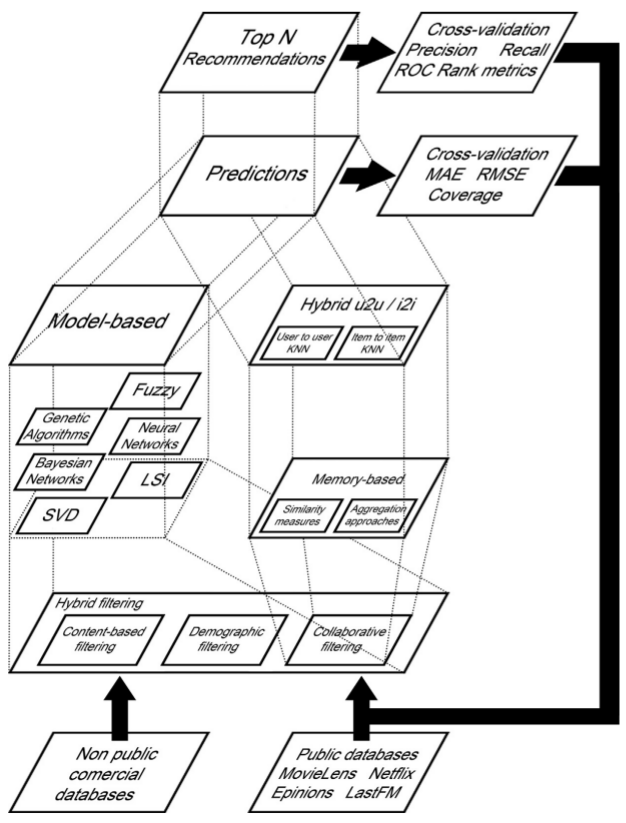
\includegraphics[scale=0.40]{images/model-recomm.png}
	\caption{Modelli di Raccomandazione \cite{Bobadilla:2013:RSS:2483330.2483573}}
	\label{model-rec}
\end{figure}

E' utile citare i metodi di riduzione basati sulla Matrix Factorization, la tecnica model-based Latent Semantic Index (LSI), il metodo di riduzione Singular Value Decomposition
(SVD) e le tecniche di clustering.

Nella Figura \ref{model-rec} viene illustrato un diagramma con le tecniche principali e gli algoritmi di raccomandazione maggiormente utilizzati in letteratura \cite{Bobadilla:2013:RSS:2483330.2483573}.

\subsubsection{Metriche di Valutazione}
La qualità di un sistema di raccomandazione può essere valutata dai risultati forniti in output. Le tipologie di metriche usate, dipendono dal tipo di CF usato. Le metriche possono essere categorizzate in:
Predictive Accuracy, come ad esempio il Mean Absolute Error
(MAE) e sue varianti; Classification Accuracy metrics, come la precision, recall, F1-measure, e sensibilità ROC; Rank Accuracy, come il Mean Average Precision (MAP), e così via.
Desideriamo concentrarci sulla metrica \textbf{Root Mean Squared Error} (RMSE). Infatti la radice quadrata dell'errore quadratico medio, è una metrica molto utilizzata per la raccomandazione di film.

\[ RMSE=\sqrt{\frac{1}{n}\sum_{{i,j}}(p_{i,j}-r_{i,j})^2} \]

dove $n$ è il numero totale dei voti assegnati dagli utenti,$p_{i,j}$ è il voto predetto per l'utente $i$ sull'elemento $j$, ed $r_{i,j}$ è il voto attuale. L'RMSE consente di valutare in maniera precisa i contributi degli errori assoluti tra i valori predetti ed i valori reali \cite{Su:2009:SCF:1592474.1722966}.
\subsubsection{Filtro collaborativo}

\subsubsection{L'algoritmo ALS}

\subsection{Introduzione allo Stream Processing}
\subsubsection{Il paradigma Publish-Subscribe}
\subsection{Il pattern Facade}
\subsection{Il pattern Singleton}
\subsection{Il pattern Model-View-Controller (MVC)}
\subsection{La tecnologia WebSocket}

\section{Analisi del progetto}

\section{Soluzione proposta}

\subsection{La libreria Spark}

Apache Spark è un sistema di cluster computing di tipo general-purpose, scalabile e veloce. Dispone di API di alto livello in \textbf{Java}, \textbf{Scala},\textbf{ Python} ed \textbf{R}, e un engine ottimizzato che supporta grafi di esecuzione generici. Supporta inoltre un ampio set di tool come \textbf{Spark SQL}, per structured data processing, \textbf{MLlib} per il machine learning e \textbf{Spark Streaming}, descritti nelle sezioni successive. Spark è eseguibile sia su sistemi Windows che UNIX-like (Linux, Mac OS). \\

Una delle possibili configurazioni di un sistema Spark è la modalità \textit{cluster}, mostrata in Figura \ref{spark-cluster}. 

\begin{figure}[H]
	\centering
	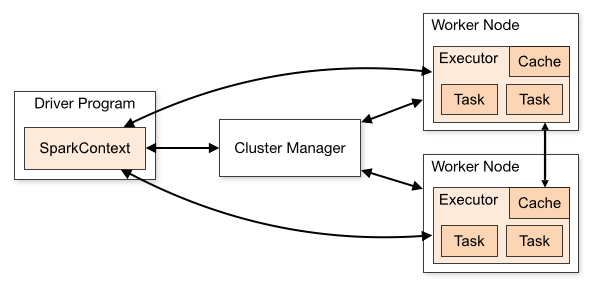
\includegraphics[scale=0.50]{images/cluster-overview.png}
	\caption{Configurazione in Spark di tipo Cluster Mode}
	\label{spark-cluster}
\end{figure}

Le applicazioni Spark sono eseguite come un set di processi indipendenti sul cluster, coordinati dall'oggetto \textit{SparkContext} del programma sorgente (detto \textbf{driver program}). Precisamente, il programma driver può connettersi su diversi tipi di \textit{cluster managers} (ad esempio un cluster di tipo Standalone, Mesos o YARN), il quale alloca le risorse a disposizione delle applicazioni. Una volta connesso, Spark scansiona i nodi del cluster alla ricerca degli \textbf{executor} (detti anche \textit{worker node}), i quali eseguono effettivamente i task e il data storage delle applicazioni. A questo punto il driver invia il codice dell'applicazione agli executor (tipicamente un file JAR o file Python incluso nello SparkContext) e schedula i task per l'esecuzione parallela. 

Alcune considerazioni riguardo tale architettura sono: 
\begin{itemize}
	\item Ogni applicazione gestisce i propri workers, i quali restano attivi durante tutto il ciclo di vita ed eseguono task multipli in thread multipli. Questo implica un isolamento tra le applicazioni, sia lato scheduling (ogni driver schedula i propri tasks) sia lato executor (tasks relativi ad applicazioni differenti risiedono in JVM differenti). Tuttavia ciò implica che non è possibile condividere nativamente i dati tra applicazioni diverse, a meno di utilizzare uno storage system esterno.
	\item Il driver deve poter gestire le connessioni con i workers durante l'intero ciclo di vita dell'applicazione. Per questo motivo dev'essere sempre garantita la visibilità a livello di rete tra driver e workers durante l'esecuzione.
	\item \`E necessario che driver e worker abbiano, a livello di rete, una distanza relativamente breve, preferibilmente nella stessa LAN, affinché lo scheduling sia rapidamente eseguito. 
\end{itemize}

Il principio di funzionamento di Spark si basa sostanzialmente sul concetto di \textit{Resilient Distributed Dataset} (\textbf{RDD}). Un RDD è una collezione di dati su cui è possibile operare parallelamente, ed è distribuita su tutti i nodi del cluster come file system Hadoop oppure è generata da una collezione esistente in Java o Scala. \\

Una seconda astrazione è rappresentata dalle variabili condivise (\textit{shared variables}), utilizzate nelle computazioni parallele. Di default Spark tiene traccia delle variabili istanziate nei vari task, e consente se necessario di condividerle fra task o fra task e driver. Le variabili condivise possono essere di due tipi: di tipo \textit{broadcast}, il cui valore viene salvato nella cache per ogni nodo, e di tipo \textit{accumulatore}, per esempio contatori o sommatori.

\subsubsection{Spark Streaming}

Spark Streaming è un'estensione delle Core API di Spark per lo\textbf{ stream processing} di live data streams ad alto throughput. Supporta molteplici sorgenti di data stream come\textbf{ Kafka}, Flume, Twitter, ZeroMQ, Kinesis o socket TCP, i quali possono essere processati tramite direttive come \textit{map}, \textit{join}, \textit{reduce} e \textit{window}. Nel post processing è possibile salvare i data stream in un file system, in un database o visualizzarli in una live dashboard. Come ulteriore fase nella pipeline di operazione rientra anche il machine learning ed il graph processing. In Figura \ref{spark-streaming} viene riassunta l'architettura descritta. 

\begin{figure}[H]
	\centering
	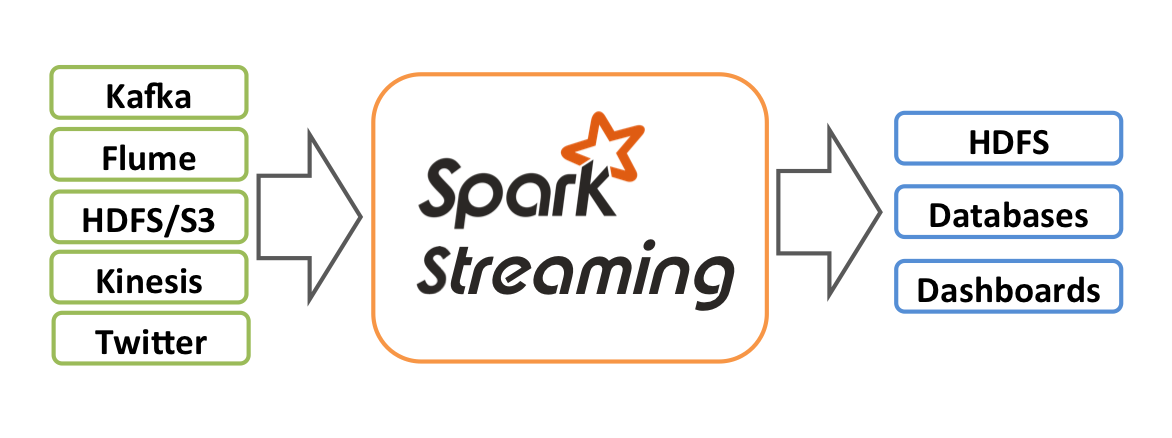
\includegraphics[scale=0.50]{images/streaming-arch.png}
	\caption{Architettura di Spark Streaming}
	\label{spark-streaming}
\end{figure}

Nello specifico, i data streams ricevuti vengono suddivisi in frammenti (\textit{batches}), processati da Spark per generare lo stream finale risultante in batches, come mostrato in Figura \ref{spark-streaming-processing}.

\begin{figure}[H]
	\centering
	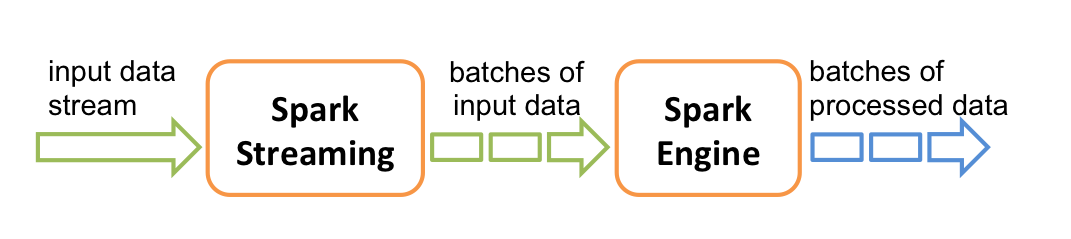
\includegraphics[scale=0.50]{images/streaming-flow.png}
	\caption{Spark Streaming Data Stream Processing}
	\label{spark-streaming-processing}
\end{figure}

A livello alto il flusso continuo di dati è rappresento da una struttura astratta detta \textit{discretized stream} o \textit{DStream}, il cui contenuto è rappresentato da tutte le sorgenti collegate eventualmente con Spark, o da stream risultati da altri DStream. Internamente, un DStream è rappresentato tramite una sequenza di RDD. 

\subsubsection{Spark MLlib}
\subsubsection{Spark SQL}

\subsection{Apache Kafka}
\subsubsection{Panoramica}
\subsubsection{Integrazione con Spark Streaming}

\subsection{Il framework Node.js}
\subsubsection{Panoramica}
\subsubsection{Kafka Client per Node.js}
\subsubsection{Il framework Angular.js}
\subsection{La libreria socket.IO}

\section{Conclusioni e sviluppi futuri}

\clearpage
\addcontentsline{toc}{section}{Bibliografia}
\nocite{*}
\bibliographystyle{plain}
\bibliography{biblib}


\end{document}